\section{Introduction}

% ------------------------------------------------------------------------------
% src: figures/df_intro_time.pdf <- juliet_full/analysis/deadfree/latency_deadfree.csv (median_s, latency300 DeadFree
%   units, concurrency 1); grey "pending" bars until the latency-deadfree lane writes the file.
\begin{frame}{Leak checks must fit a developer's time budget}
  \centering
  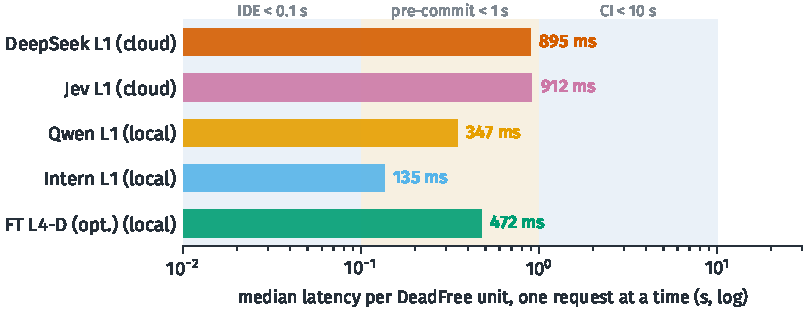
\includegraphics[width=\linewidth,height=0.60\textheight,keepaspectratio]{figures/df_intro_time.pdf}\\[4pt]
  \begin{tabular}{@{}ccc@{}}
    IDE: $<$\,0.1\,s & \quad pre-commit: $<$\,1\,s & \quad CI: $<$\,10\,s \\
  \end{tabular}
  \vfill
  {\scriptsize Cloud: DeepSeek V4.1 Flash API, Jev decision API (network round-trip). Local: one RTX 3090 (24\,GB).
  Median per DeadFree unit, one request at a time, same client.\par}
\end{frame}

% ------------------------------------------------------------------------------
% src: figures/df_intro_quality.pdf <- juliet_full/analysis/deadfree/deadfree_quality.json (macro_f1, eval 2,656 units)
\begin{frame}{On DeadFree, cloud models are far ahead of local ones}
  \centering
  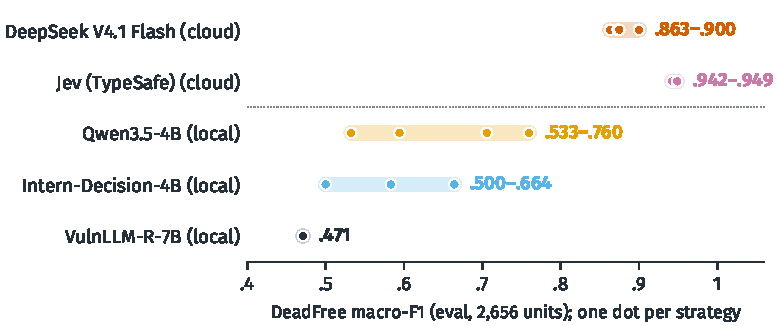
\includegraphics[width=\linewidth,height=0.60\textheight,keepaspectratio]{figures/df_intro_quality.pdf}\\[4pt]
  {\small Cloud \res{df-deepseek_L1}{macro}--\res{df-jev_L3}{macro};
  best untuned local prompt (L1--L4): Qwen L3 \res{df-qwen_L3}{macro}; VulnLLM-R-7B (vulnerability-tuned): \res{df-vulnllmr}{macro}\par}
  \vfill
  {\scriptsize DeadFree: Juliet CWE-401 units with a \code{free} that never runs (method section). Macro-F1, leak = positive class.\par}
\end{frame}

% ------------------------------------------------------------------------------
% src: figures/hook_original.pdf <- juliet_full/data/build/probes.json (static void) and registry runs on layer "original"
\begin{frame}{Original Juliet can be gamed: a one-line rule beats Clang SA}
  \begin{columns}[c]
    \begin{column}{0.57\textwidth}
      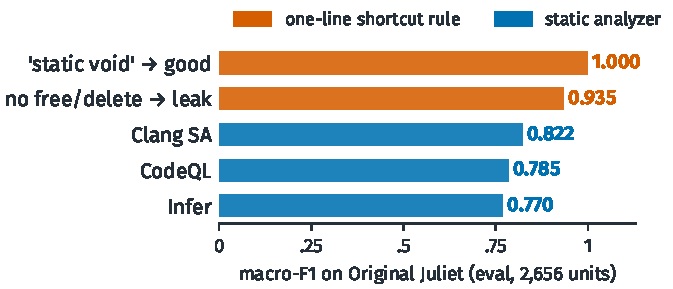
\includegraphics[width=\linewidth]{figures/hook_original.pdf}
    \end{column}
    \begin{column}{0.41\textwidth}
      \begin{itemize}
        \item ``no \code{free}/\code{delete} $\Rightarrow$ leak'': \res{grep-original}{macro}
        \item ``has \code{static void} $\Rightarrow$ good'': \res{x}{probe_static_void_original}
        \item Clang SA: \res{clang_sa-original}{macro}
      \end{itemize}
      \vspace{6pt}
      \alert{Templates reveal the label.}
    \end{column}
  \end{columns}
  \vfill
  {\scriptsize Template shortcuts: Germano et al.\ (ICAART'25); Risse \& B\"ohme (USENIX Sec'24).\par}
\end{frame}

% ------------------------------------------------------------------------------
\begin{frame}{Question: near-cloud quality on a local device?}
  \centering
  \begin{tikzpicture}[node distance=5mm and 8mm]
    \node[warn, minimum width=46mm, minimum height=14mm] (cloud) {\textbf{Cloud}\\{\small accurate, slow, paid}};
    \node[data, right=22mm of cloud, minimum width=46mm, minimum height=14mm] (local) {\textbf{Local 4B model}\\{\small fast, free, weak}};
    \draw[arr, dashed] (local.west) -- node[lbl, above] {close the gap?} (cloud.east);
  \end{tikzpicture}
  \vspace{10pt}
  \begin{enumerate}
    \item Which \textbf{strategy} helps a local model most?
    \item Does \textbf{fine-tuning} help, and on which labels?
    \item How close to the cloud do we get, and how fast?
  \end{enumerate}
  \vspace{4pt}
  {\small Task: one Juliet CWE-401 unit (C/C++) $\to$ leak / no leak, judged on \textbf{DeadFree}.\par}
\end{frame}
